\documentclass{rapport}
\usepackage[utf8]{inputenc}

\usepackage{pifont} % Pour les symboles appelés par la macro \ding
\usepackage{url} % Comme son nom l'indique, pour les url...

\usetikzlibrary{positioning} % Bibliothèque tikz pour positionner des nœuds relativement à d'autres

\usepackage[colorlinks, citecolor=red!60!green, linkcolor=blue!60!green, urlcolor=magenta]{hyperref} % Pour que les liens soient cliquables. Les options permettent de mettre les liens en couleur.

\usepackage{algorithm}
\usepackage{algo}
\usepackage{colorationSyntaxique}
\usepackage{listings}
\usepackage{graphicx}
\usepackage{float}


% Pour un rapport en français 
% \usepackage[francais]{babel} % Commenter pour un rapport en anglais
% \renewcommand\bibsection{\section*{Bibliographie}} % Commenter pour un rapport en anglais

\englishTitlePage % Décommenter pour une page de titre en anglais


\pagestyle{fancy}
\renewcommand{\sectionmark}[1]{\markboth{\thesection.\ #1}{}}
\fancyfoot{}

\newcommand{\gcc}{\texttt{gcc} }
\newcommand{\icx}{\texttt{icx} }
\newcommand{\clang}{\texttt{clang} }
\newcommand{\comp}{\texttt{ccomp} }
\newcommand{\optizero}{\texttt{-O0} }
\newcommand{\optione}{\texttt{-O1} }
\newcommand{\optitwo}{\texttt{-O2} }
\newcommand{\optithree}{\texttt{-O3} }
\newcommand{\optisize}{\texttt{-Os} }

\fancyhead[LE]{\textsl{\leftmark}}
\fancyhead[RE, LO]{\textbf{\thepage}}
\fancyhead[RO]{\textsl{\rightmark}}

\def\Latex{\LaTeX\xspace}
\def\etc{\textit{etc.}\xspace}

\lstset{                  % Specify language
basicstyle=\ttfamily\small,     % Code font and size
keywordstyle=\color{blue},      % Color for keywords
commentstyle=\color{gray},      % Color for comments
stringstyle=\color{red},        % Color for strings
numbers=left,                   % Add line numbers
numberstyle=\tiny\color{gray},  % Style for line numbers
% frame=single,                   % Add a border around code
breaklines=true,                % Line wrapping
% backgroundcolor=\color{gray!10} % Light gray background
}


\title{Optimizing application performance through optimizing compilation}
\author{Francois Flandin}
\supervisor{Pr Sid Touati}
\date{First semester of year 2024-2025}

% \universityname{Université Côte d'Azur} % Nom de l'université.
% \type{TER} % Type de document
% \formation{Master Informatique} % Nom de la formation

% Retrouver les autres options possibles dans le document rapport.pdf

\begin{document}

\maketitle

\begin{abstract}
This report investigates the impact of compiler optimizations on application performance by comparing four compilers—\gcc, \clang, \icx, and \comp—across multiple optimization levels: 
\optizero, \optione, \optitwo, \optithree, and \optisize. 
\newline
Two programs, a matrix multiplication in \texttt{C} and Dijkstra’s algorithm in \texttt{C++}, were used to evaluate execution 
times, highlighting how different compilers handle computationally intensive tasks and memory-heavy workloads. 
\newline
The analysis shows that \gcc consistently outperforms others in \texttt{C}
tasks due to its robust optimization capabilities, while \clang excels in \texttt{C++} scenarios, leveraging its deeper understanding of modern constructs. \newline
\icx and \comp, though less performant, are designed for specific use cases like hardware-specific tuning and formally verified code, respectively. \newline
The findings emphasize the importance of choosing the right compiler for specific tasks and suggest directions for further research, including energy-efficient 
optimizations and real-world mixed-language applications.
\end{abstract}

\clearpage

\tableofcontents

\clearpage
% \section*{Summary}
% \addcontentsline{toc}{section}{Summary}
% This report investigates the impact of compiler optimizations on application performance by comparing four compilers—\gcc, \clang, \icx, and \comp—across multiple optimization levels: 
% \optizero, \optione, \optitwo, \optithree, and \optisize. 
% \newline
% Two programs, a matrix multiplication in \texttt{C} and Dijkstra’s algorithm in \texttt{C++}, were used to evaluate execution 
% times, highlighting how different compilers handle computationally intensive tasks and memory-heavy workloads. 
% \newline
% The analysis shows that \gcc consistently outperforms others in \texttt{C}
% tasks due to its robust optimization capabilities, while \clang excels in \texttt{C++} scenarios, leveraging its deeper understanding of modern constructs. \newline
% \icx and \comp, though less performant, are designed for specific use cases like hardware-specific tuning and formally verified code, respectively. The findings emphasize the importance 
% of choosing the right compiler for specific tasks and suggest directions for further research, including energy-efficient optimizations and real-world mixed-language applications.

\clearpage

\section*{Introduction}
\addcontentsline{toc}{section}{Introduction}
The tutoring project titled "Optimizing Application Performance through Compilation Optimization" explores how compilers improve the generated code 
using various optimization levels: \optizero, \optione, \optitwo, \optithree, and \optisize. \newline
The different optimization levels goes from \optizero, which means no optimization, to \optithree, which enables the most optimizations, but also \optisize, which
compiles to have the most compact code.\newline
This project is divided into two main phases:
\begin{itemize}
    \item Experimentation: Compile two programs with four different compilers (\gcc, \icx, \clang, and \comp) at each optimization level, 
    measure execution times over 12 iterations, and visualize the data using \texttt{R}.
    \item Optimization Analysis: Study the optimization options enabled by each compiler at each level, to better understand their internal mechanisms.
\end{itemize}
These steps allow for the evaluation of compilers not only in terms of speed but also by identifying the specific characteristics of each optimization level.


\section*{State of the Art}
\addcontentsline{toc}{section}{State of the Art}
Compiler optimizations play a crucial role in improving program performance by transforming source code into highly efficient machine code. Modern compilers like \gcc, \clang, and \icx 
employ a range of techniques to optimize loops, eliminate redundant computations, and streamline memory usage. For example, \gcc’s loop unrolling and vectorization strategies enable 
significant performance gains in computationally intensive workloads, while \clang’s adherence to modern \texttt{C++} standards gives it an edge in handling advanced type systems and 
constructs.
\newline\newline
Despite their capabilities, these compilers face trade-offs. \gcc is known for its aggressive optimizations but may struggle with \texttt{C++}-specific features. \clang prioritizes 
modularity and diagnostics, making it a preferred choice for developers working on complex \texttt{C++} codebases. \icx, designed for Intel architectures, excels in leveraging 
hardware-specific features but shows weaker performance in general-purpose workloads. Meanwhile, \comp stands apart as a formally verified compiler, prioritizing correctness over speed, 
making it indispensable for safety-critical applications.
\newline\newline
Recent advancements in compiler technology focus on expanding interprocedural analysis, incorporating energy efficiency into optimization strategies, and enhancing debugging tools. 
However, challenges remain, such as balancing compile-time performance with runtime efficiency, ensuring cross-platform consistency, and addressing the growing demand for 
energy-efficient computing. These limitations underline the need for further research into compiler optimization techniques tailored for modern hardware and software ecosystems.
\clearpage

\part{The experience}

\section{Experience's environnement}
In this part will be presented the environnement of the experimentations, on which hardware it was done, on which software, etc.
\subsection*{Hardware}
In this part, the hardware part of the computer will be explored. \newline
To explore the hardware of a computer on linux, the folder \texttt{/cpu} can be explored, it gives us the \textit{topology} of the cpu, like which threads are on each cores, which caches are on each cores, discover what is the cache line size etc...\newline
But there are also a lot of linux tools that allows to check the hardware's specifications of a computer, and basically do the job for us. \newline
There are graphical tools such as \texttt{likwid}, which provides the command \texttt{likwid-topology}, or the tool \texttt{hwloc}, which provides \texttt{lstopo}, a command that gives a beautiful GUI of the computer's hardware's specification.
\begin{description}
    \item[Model name :] 11th Gen Intel(R) Core(TM) i5-1135G7 @ 2.40GHz
    \item[Adress size :] 39 bits physical, 48 bits virtual
    \item[Cache line size :] 64 bytes
    \item[Cores :] 4
\end{description}

\begin{table}[H]
    \centering
    \begin{tabular}{|l|c|c|c|c|}
        \hline
        \multicolumn{5}{|c|}{Graphical Topology} \\
        \hline
        Coeurs & \enspace0\enspace\enspace4 &\enspace1\enspace\enspace5 &\enspace2\enspace\enspace6 &\enspace3\enspace\enspace7 \\
        \hline
        Cache L1 & \enspace48 kB &\enspace48 kB &\enspace48 kB &\enspace48 kB \\
        \hline
        Cache L2 & 1MB & 1MB & 1MB & 1MB \\
        \hline
        Cache L3 & \multicolumn{4}{|c|}{8 MB} \\
        \hline
    \end{tabular}
    \caption{Computer's topology}
    \label{tab:graph_characteristics}
\end{table}


\subsection*{Software}
For the software part, the experiments were done on a lightweight configuration of the computer, where all unnecessary services were disabled, 
including the graphical interface, this allows the computer to run as baremetal as possible. \newline
Here is a description of all the software elements used in this benchmark :
\begin{description}
    \item[OS] Fedora Linux v40 WorkStation
    \item[gcc] version 14.2.1 20240912
    \item[icx] version 2024.2.1.20240711
    \item[clang] version 18.1.8
    \item[ccomp] version 3.14
\end{description}

\section{Experiment method}
To compare the performance of the different compilers, two programs will be used, the first \texttt{matrix\_multiply}, is a \texttt{C} program 
that multiplies two matrices to put the result in a third matrix, it is an interesting challenge for optimization because of the presence of 3 nested loops for 
the calculation. Moreover, the size of the matrix will be set to 2 times the size of the largest cache, to simulate a real-world situation, where the program would have to frequently go 
to memory to store such a wide matrix. This program will be compiled using \gcc, \clang, \icx and \comp. \newline
The second program is \texttt{dijkstra} algorithm written in \texttt{C++}, the goal behind this is to compare the compilers optimizations when the program has a lot
of memory usage, because it is in \texttt{C++}, the program will only be compiled with the \texttt{C++} versions of \gcc, \clang and \icx, due to the lack of \texttt{C++}
compilation from \comp. \newline
Next, we can mesure time taken by the program by placing the c-function \texttt{gettimeofday()} around the function that we need to calculate, initialisation 
mesurement is not the main goal, but it can be mesured too. The programs are executed 12 times for each optimization level to make an interesting violin plot using \texttt{R}.

\section{Results}
\subsection{Matrix Multiplication Results}
\begin{figure}[H]
\centering
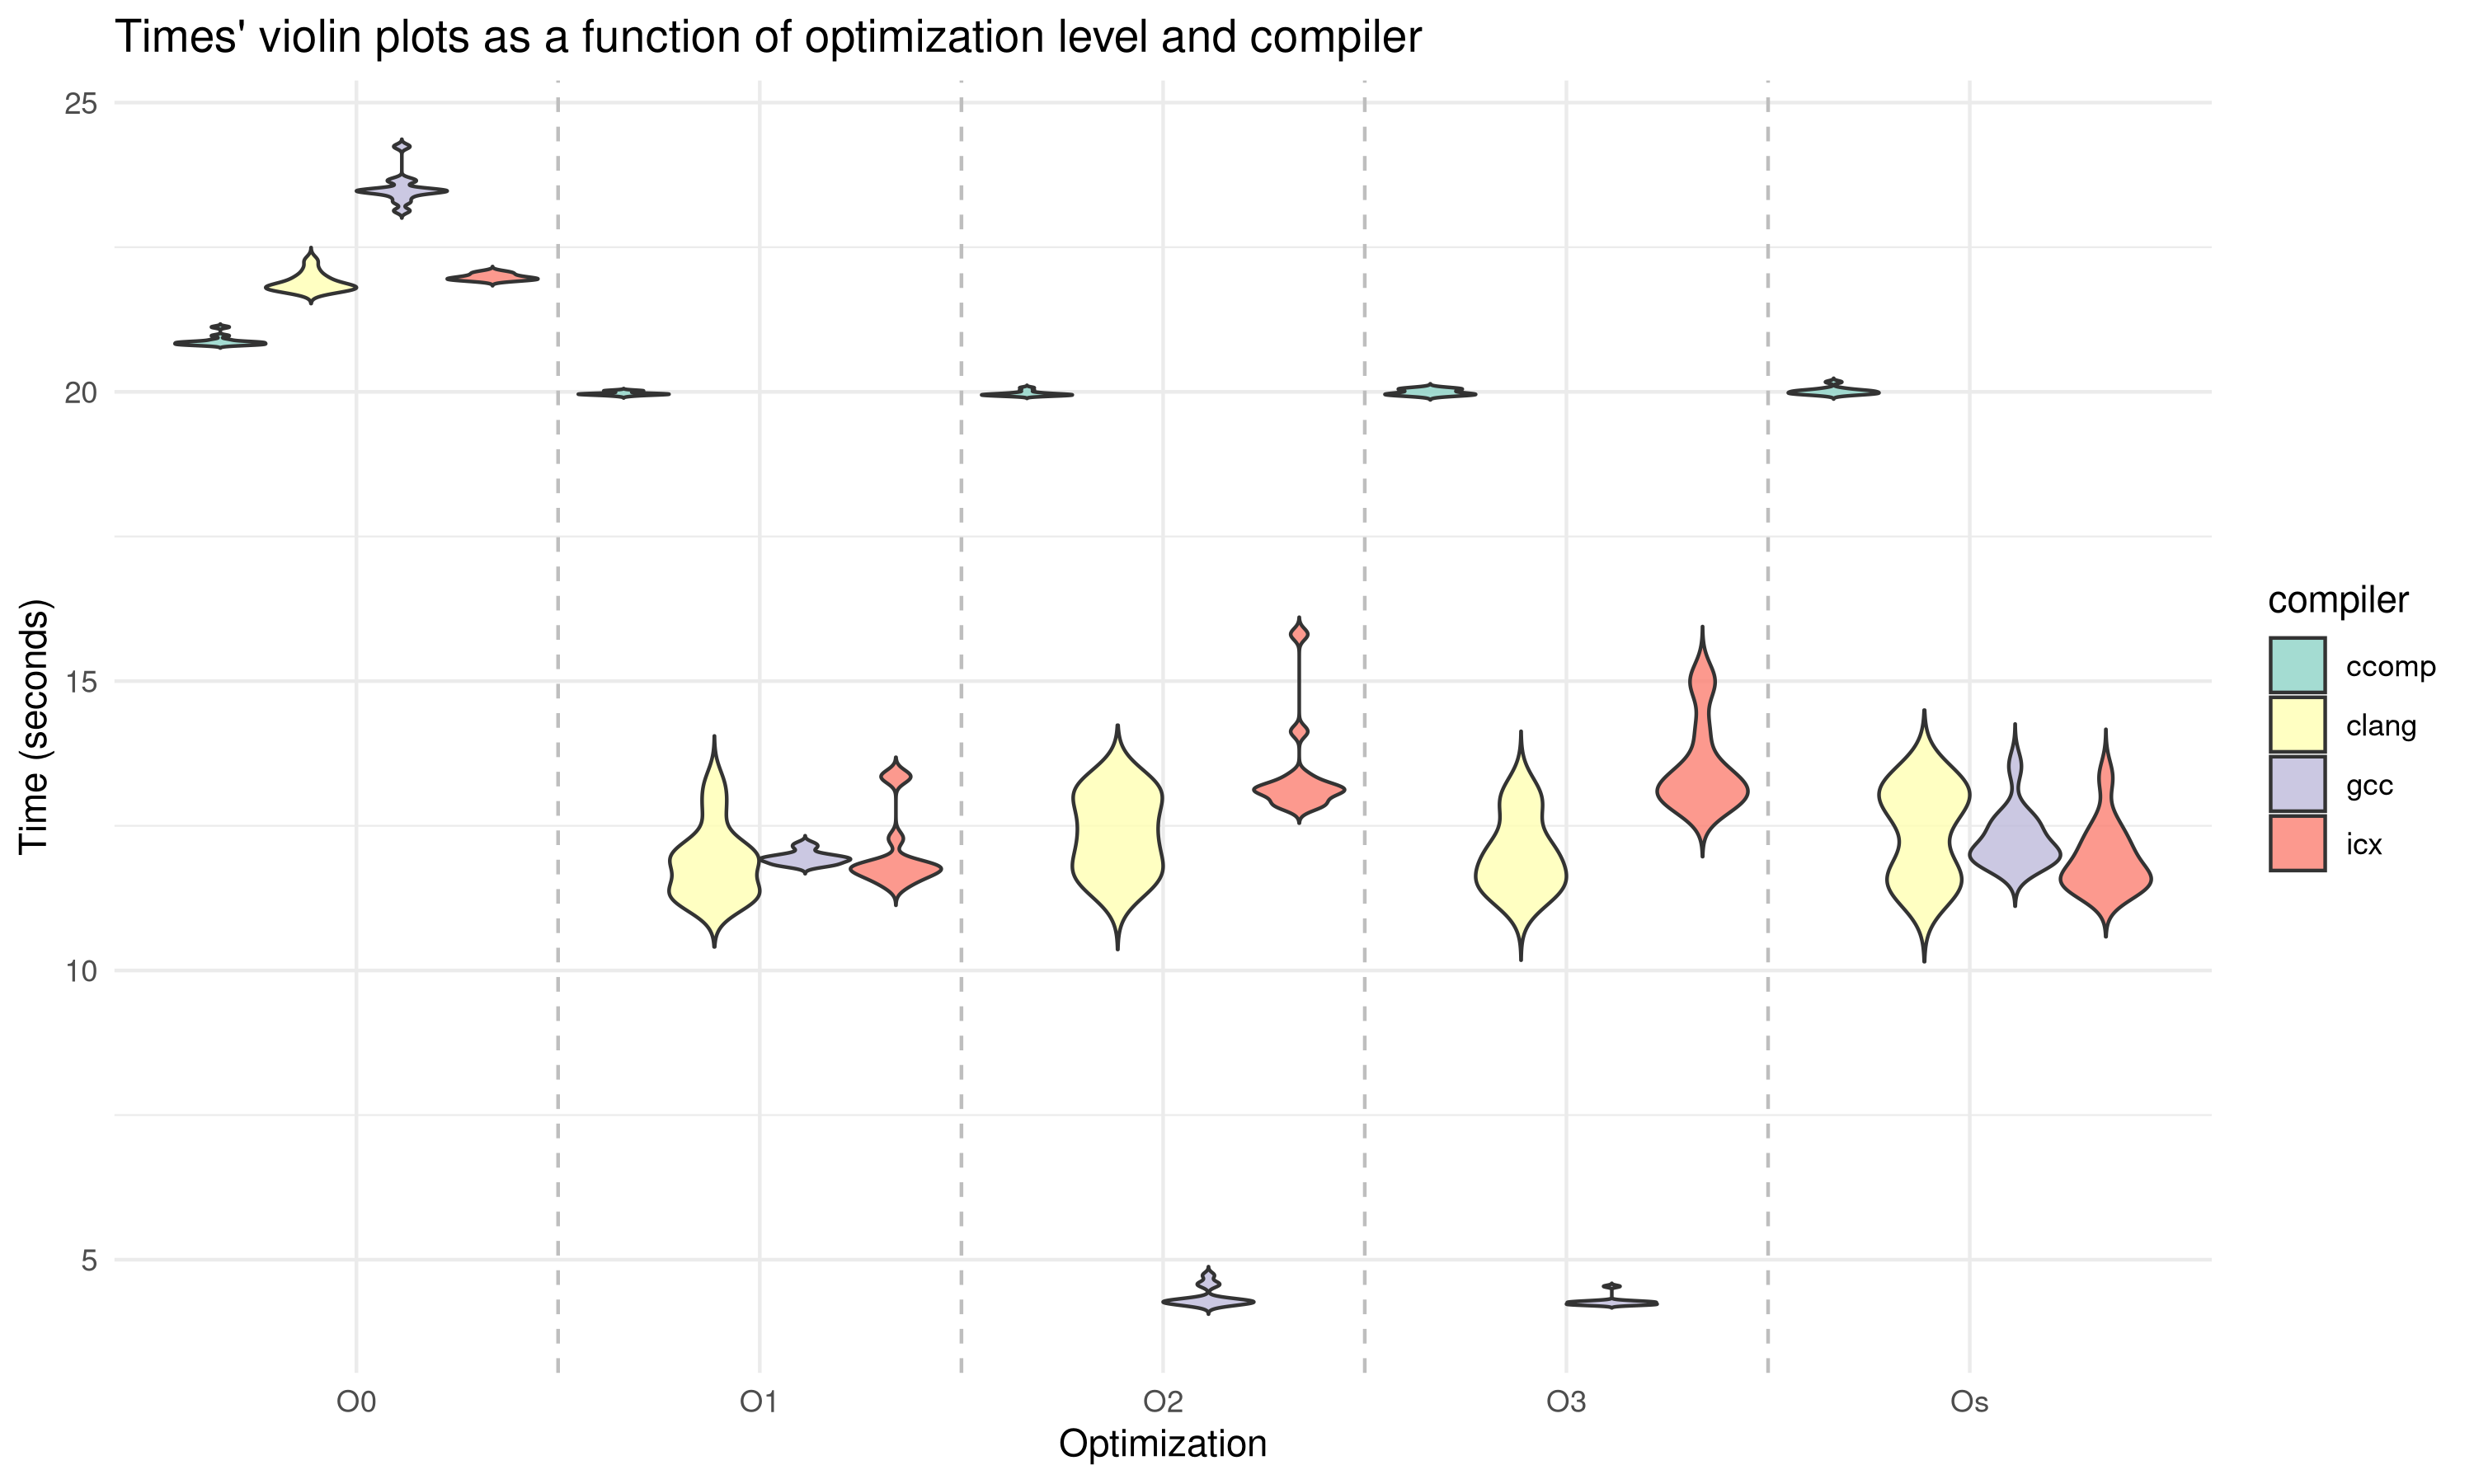
\includegraphics[width=1\textwidth]{img/plots/violin_plot_mat_mult.png}
\caption{Evolution of the execution time of the program mat\_mult.c as a function of compiler and optimization level.}
\label{fig:image1}
\end{figure}
The results for the C program (matrix multiplication) highlight clear differences in how each compiler handles optimizations.\newline
\gcc stands out as the best-performing compiler for this benchmark. It starts slower at -O0, but quickly improves with each optimization level, reaching the best execution times at 
\optitwo and \optithree. This suggests that \gcc performs transformations which deal efficiently with the nested loop structure of the matrix multiplication making it suitable for such tasks.
\newline
\clang shows a reliable improvement across optimization levels, but it remains behind \gcc. While its performance gains are noticeable, it doesn’t manage to handle the program as 
efficiently, especially at higher optimization levels. This difference suggests a less aggressive approach to handling the bottlenecks present in nested loops. \newline
Despite being developed for Intel architectures, \icx does not perform as well as expected. Its optimizations do improve execution times, but not enough to compete with \gcc or \clang. 
This makes \icx less effective for matrix-heavy computations, suggesting it might prioritize other types of workloads. \newline
\comp delivers the slowest execution times in this benchmark, which is in line with its goal of producing formally verified code. While correctness is ensured, 
performance is not a priority, and its constant execution times across optimization levels reflect this limitation.

\subsection{Dijkstra Results}
\begin{figure}[H]
\centering
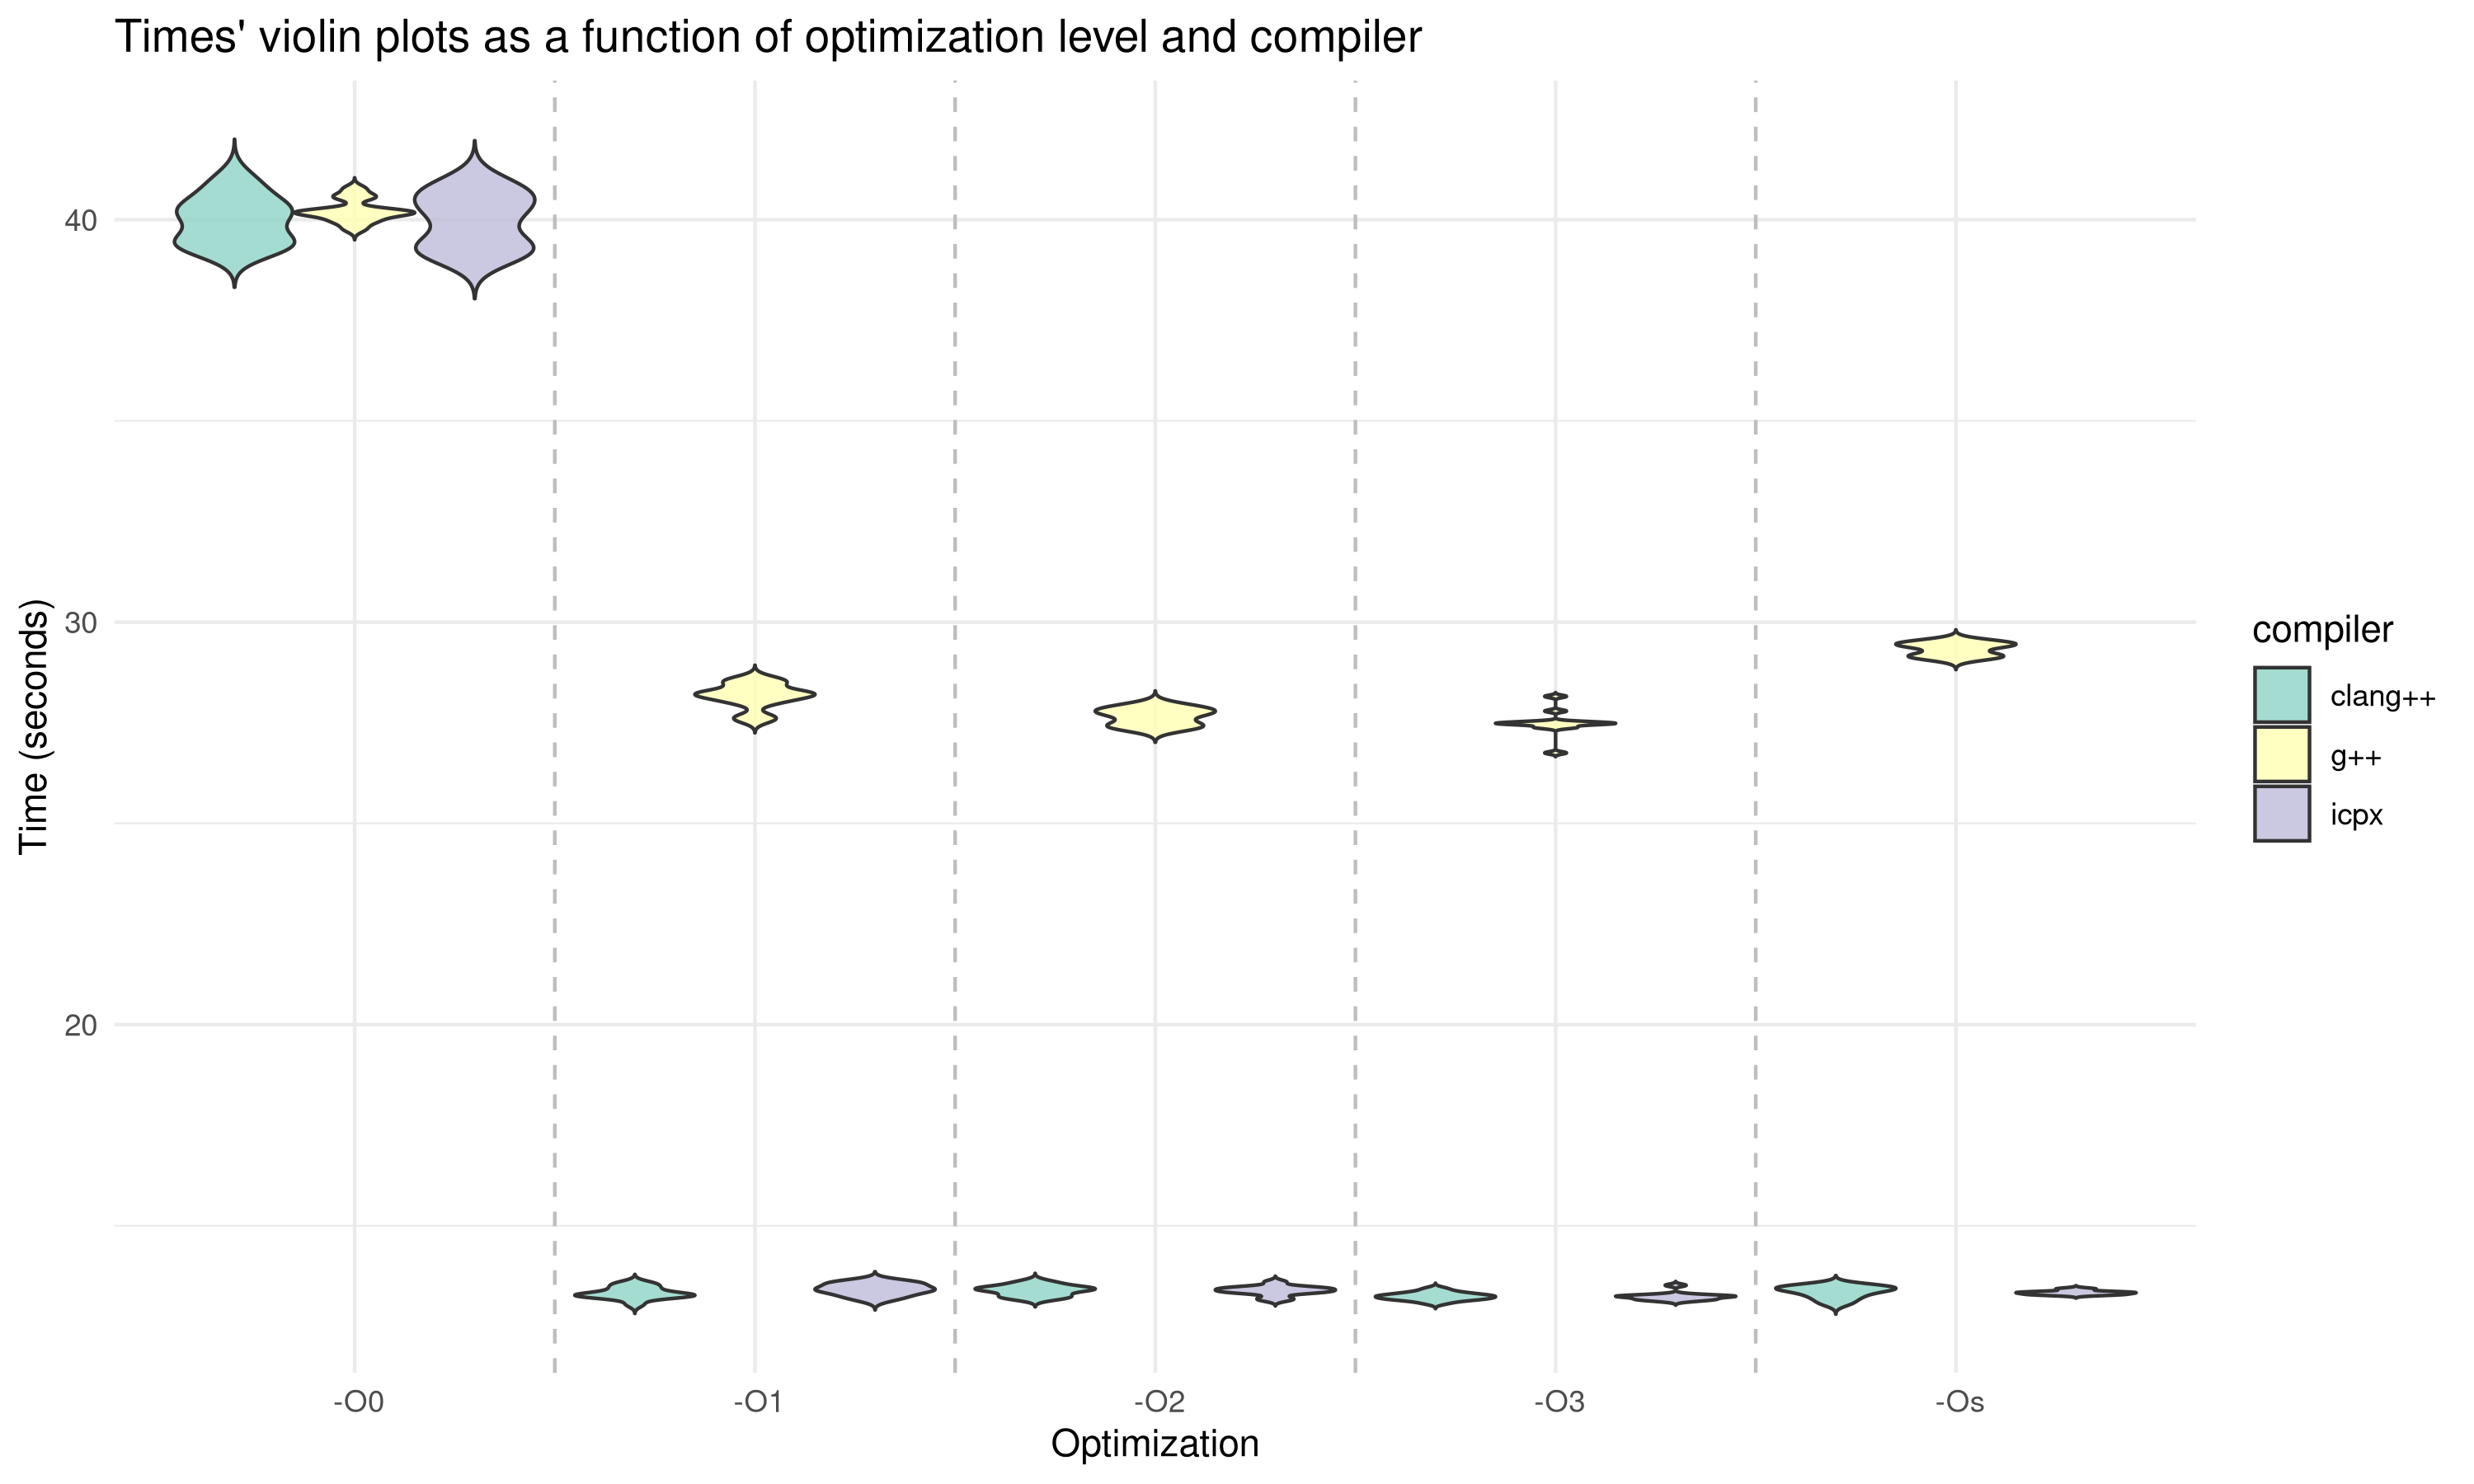
\includegraphics[width=1\textwidth]{img/plots/violin_plot_dijkstra.png}
\caption{Evolution of the execution time of the program dijkstra.cpp as a function of compiler and optimization level.}
\label{fig:image2}
\end{figure}
What we can notice from these 2 graphs, is how differently \gcc compares with \clang and \icx according to the language used, \texttt{C} or \texttt{C++}. 
When using \texttt{C}, \gcc produces way more optimized codes than \clang and \icx, whereas in \texttt{C++}, \gcc is the least performant one. \newline
Few experiments were done get some answers to why is it like this. \newline\newline
First, the experiments were made on the \texttt{C++} programs, at the compilation level of \optithree, this will give us some data to work with, and, 
by using the command \texttt{perf record} and \texttt{perf report}, we can use material performance counters to get a lot of data on the percentage of time used 
by a function, we could use profiling applications such as \texttt{gprof}, but \texttt{perf} allowed us to have more precise data and avoided us to recompile
entirely the program.\newline \newline
The results were the following:
\begin{table}[H]
\centering
\begin{tabular}{|l|c|c|c|}
\hline
                           & \gcc    & \clang  & \icx   \\
\hline
total time taken & 136.37s       & 146.98s       & 155.65s \\
dijkstra usage   & $\approx26s$  & $\approx13s$  & $\approx17s$    \\
init/free usage  & $\approx109s$ & $\approx133s$ & $\approx138s$   \\
\hline
\end{tabular}
\end{table}
What we can get as results from here is that \gcc is the most optimized in terms of initialisation and memory management, but is the worst one in terms 
of pure dijkstra calculation. \newline
If we push further the analysis, we can see there are some points in the program where types inference were used, such as \texttt{for (auto edge : temp\_neighbors)}. 
\gcc might not be able to manage this type system as well as \clang or \icx, hence the lack of optimizations.

\clearpage
\part{Compilers}
In this part will be presented all the compilers used in this tutorship project, as well as deepening their optimization options for each optimizations levels.
\newline
The optimizations presented are not exhaustive, only the most importants will be presented, and the method to obtain the optimizations will be given
for each compiler, so the experiments can be reproduced.




\section{\gcc}
\gcc is the most popular \texttt{C} compiler, it comes in the \texttt{GNU Compiler Collection}, which includes compilers for \texttt{Fortran}, \texttt{C++}, \texttt{Go}...

\subsection*{Optimizations Obtention Method}
\gcc is really helpful regarding getting informations about what he does, because the compiler has an option for this sole purpose, which is
\begin{verbatim}
gcc --help=optimizers -Q -On
\end{verbatim}

\subsection*{Optimizations introduced by \optizero}
\gcc \optizero was originally meant to disable every optimization flags to give the least optimized code, however, the competition with other compilers led to 
now have some optimization flags enabled, 53 to be more precise. For the most, optimizations at this level are analysis options.
\newline\newline
A part of the optimizations concerns loop optimizations, with the option \newline \texttt{-faggressive-loop-optimizations}, \gcc enables, as its name suggests, a lot of loop optimizations, 
such as \textbf{loop unrolling}, which reduces loop overhead by duplicating the loop body multiple times, minimizing the number of iterations and improving execution efficiency, 
\textbf{loop fusion}, which combines loops that access the same data into a single loop, reducing overhead from multiple passes over the data, or \textbf{loop peeling}, which moves loops
special cases outside of the loop. \newline\newline
Next is the dead code elimination, \gcc can also remove every line of code that isn't used, this doesn't impact the execution speed, but reduces the size of the generated code.\newline
And finally are the peephole optimizations this option introduces optimizations on a reduced window, optimizing redundant register moves, redundant calculations, etc.
\newline
Other enabled options at \optizero are either analysis options or add error-handling instructions.

\subsection*{Optimizations introduced by \optione}
\textbf{Intermediate Tree Optimizations} \newline
\gcc \optione optimizations add optimizations to the tree that the compiler builds in the intermediate level.
\newline
First, there is the dead code and redundancy elimination, with the options \texttt{-ftree-dce}, \texttt{-ftree-fre} and \texttt{-ftree-dse}, \gcc removes all the \textbf{dead code}, 
computations that produce the same results as well as all \textbf{dead stores}, that means that the cpu has less operations to manage, and the code size is reduced.
\newline
Secondly, there is value and copy propagation, first, the option \texttt{-ftree-ccp} tells the compiler to propagate constant values across conditions when it's possible, 
it simplifies all the control flow and makes place for further optimizations, and can even help for \texttt{branch prediction}. \newline Secondly, the option \texttt{-ftree-copy-prop} 
propagates values with copy instructions, for example \texttt{b = a; c = b;} would be replaced with \texttt{c = a;}.
\newline
And finally, loop optimizations, there are two main options here to consider, the first, \texttt{-ftree-sink} moves computations outside of the loop when it's possible, it allows to 
avoid computing the same thing over and over. \newline
The second is \texttt{-ftree-sra} for \textit{scalar replacement of aggregates}, it breaks structures and array into individual variable when needed, it can improve register usage and 
enable even further optimizations. An example of this would be a variable of the struct \texttt{Point \{int x; int y\}} would be transformed from \texttt{Point p;} to 
\texttt{int p\_x, p\_y;}.
\newline\newline
At \optione, there are also other options to enable inlining of functions, that means that a function call will be replaced by the function's body, which allows for further optimizations.

\subsection*{Optimizations introduced by \optitwo}
\textbf{Interprocedural Analysis Optimizations} \newline
\gcc \optitwo introduces \texttt{IPA} (Interprocedural Analysis) optimizations, which aim to improve performance by analyzing and optimizing across function boundaries. 
This includes \texttt{-fipa-icf} (Identical Code Folding), which detects and merges functions or read-only variables with identical implementations, reducing code size and memory usage. 
\newline
Additionally, \texttt{-fipa-cp} (Constant Propagation) propagates constant values across function calls, allowing the compiler to simplify computations and eliminate unnecessary branches. 
These optimizations are particularly effective in programs with repetitive patterns or predictable input values, contributing to leaner and faster executables.
\newline
\newline
\textbf{Aligning}\newline
\gcc \optitwo introduces aligning of functions, jumps, labels, and loops, the aligning allows to ensures that the instructions fit at the beginning of cache lines, which can reduce 
cache misses. Also, aligning labels and jumps allows to decrease branch prediction misses.
\newline\newline
\optitwo also enables \texttt{-funroll-loops}, which performs loop unrolling when iteration count is known, which allows the compiler to optimize as it wishes.

\subsection*{Optimizations introduced by \optithree}
\textbf{Loop Optimizations} \newline
\gcc \optithree enables mostly further loops optimizations, such as \texttt{loop peeling}, \texttt{loop jamming}, which combines independent loops (that may or may not access the 
same data) into a single loop, and is generally combined with \texttt{loop unrolling}.\newline
\texttt{loop interchange}, which swap two loops in a nested loop, this allows to put the most changing variable to the consecutive elements in memory, instead of having the most 
changing variable to separate elements in memory, it's very useful in programs such as \texttt{matrix multiplication}. 
\newline
Finally, \texttt{loop splitting} allows simplification of a loop 
by dividing it into several loops, it simplifies the loops with the pattern \texttt{for (int $i=0$; $i<10$; $i++$) if($i<5$)... else...} into two loops, one with the range 0..4 and 
the other 5..9. It helps in reducing dependencies.

\subsection*{Optimizations enabled by \optisize}
\gcc \optisize enables the same options as \gcc \optitwo, but removes the aligning optimizations to free some space.






\section{\icx}
It's Intel's compiler for their x86 architecture, it is made to deliver extremely optimized programs on their processor architecture.
\subsection*{Optimization Obtention Method}
Everything is available in the online documentation, it's relatively easy to find what we need.
\subsection*{Optimizations introduced by \optizero}
Everything is disabled at \optizero.
\subsection*{Optimizations introduced by \optione}
At this level of optimization, \icx starts by introducing \textbf{data flow analysis}, to help gathering data about data flows throughout the whole program, 
allowing for optimizations.\newline
Then, the compiler can also reorganize code as he wishes with \textbf{code motion}, which allows to move non-changing result operations out of loop to avoid 
recomputing it over and over, and \textbf{instruction scheduling}, which allows to change the order of instructions, to hide memory latency for exemple, 
or working on a task while a heavier task is done. It is done to reduce CPU stall.
\newline\newline
Other optimizations are also enabled, \textbf{strength reduction}, that changes heavy operations for cheaper ones, like switching from a multiplication to a bit shift, \textbf{test replacement}, that simplifies loops' conditions for example : 
\begin{verbatim}
    if (x >= 0 && x < 100) { /* code */ } // base loop
    if ((unsigned)x < 100) { /* code */ } // optimized loop
\end{verbatim}
And, finally, \textbf{split-lifetime analysis}, can split the \textit{lifetime} of a variable into smaller lifetimes, to reallocate the registers when the variable is not used anymore.

\subsection*{Optimizations introduced by \optitwo}
At this level of optimization, \icx introduces more optimizations, like \textbf{constant propagation}, or \textbf{forward substitution}, which can replace variable with their expressions, for example : 
\begin{verbatim}
    int a = 5 + i
    int b = a + 3
\end{verbatim}
will be replaced by
\begin{verbatim}
    int b = 5 + i + 3
\end{verbatim}
These two options complete each other really well, because imagine that the variable \texttt{i} was a constant, it would be replaced by its value, hence further optimizing the program.
\newline\newline
Additionnal optimizations are introduced, like \textbf{loop unrolling}, \textbf{peephole optimizations}, which examines small code fragments to identify and replace inefficiencies,
such as redundant instructions or suboptimal sequences, improving code quality. Or even \textbf{optimized code selection}, which replaces inefficient instructions or code sequences with 
more efficient alternatives.
\newline\newline
There are also code-removing optimizations such as \textbf{dead-code elimination}, \textbf{dead-store elimination}, and \textbf{dead static function elimination} which does not really improves performance but can help reduce the CPU stall.

\subsection*{Optimizations introduced by \optithree}
It enables all the same optimizations as \optitwo but add more aggressive loop transformations such as \textbf{loop fusion}, \textbf{block-unroll-and-jam}, with these two options, the compiler expands and find the best fusions/jams in the loops and \textbf{collapsing-IF-statements}, where multiple successive if are combined into one to reduce branching therefore gaining performances.

\subsection*{Optimizations introduced by \optisize}
The documentation doesn't provide any information about it, except the usual "like \optitwo but optimizes for code size".















\section{\comp}
\textit{Certified Compiler}\newline
It's the only C compiler that is formally verified to produce a code described by the source code, optimized or not. By its formally verified nature, it is 
the one that produces the most inefficient code. It is generally used for safety critical programs where a bug introduced by compilation could lead to serious 
problems.

\subsection*{Optimization Obtention Method}
Everything is available in the online documentation, it's relatively easy to find what we need.
\subsection*{Optimizations introduced by \optizero}
\comp doesn't enable anything at \optizero, and the main optimization level \texttt{-O} gives the same optimizations as \optione, \optitwo, \optithree, because they are just an alias of that optimization option.
\subsection*{Optimizations introduced by \optione,\optitwo,\optithree}
There are not a lot of options so here is a list of them

\begin{description}
    \item[-fcont-prop] enables constant propagation, a process that replaces variables with their known constant values throughout the program.
    \item[-fcse] activates the elimination of common subexpressions, reducing redundant calculations by reusing previously computed values.
    \item[-fif-conversion] with this option, the compiler decides whether to replace simple if-then-else statements or the conditional operator (?:) with conditional assignements.\newline
    The heuristic-based approach selectively optimizes small and balanced expressions, provided the target architecture supports a suitable conditional move instruction.
    \item[-finline]  enables or disables the inlining of functions, potentially improving performance by replacing function calls with the actual function code.
    \item[-finline-functions-called-once] specifically inlines functions that are called only once, reducing overhead while maintaining efficiency.
    \item[-fredundancy] activates the elimination of redundant computations and unnecessary memory stores, improving execution time by avoiding repetitive operations.
    \item[-ftailcalls] optimizes function calls in tail position, which can enhance performance by reusing the current function’s stack frame. 
    \item[-ffloat-const-prop 2] enables full propagation of floating-point constants, ensuring arithmetic is performed in IEEE double precision format with round-to-nearest mode.
\end{description}

\subsection*{Optimizations introduced by \optisize}
The documentation doesn't give a lot of informations about it. Just the usual "optimizes for code size".

\section{\clang}
It's a compiler made by the LLVM Developer Group, it can replace \gcc by supporting most of the option flags of \gcc. \newline
The objective behind this compiler is to create a compiler that allowed: first, better diagnostics, which allows to debug more easily, second, to be seperated from the GNU licence, which forced
softwares to be integrated to said licence and therefore having to open\-source proprietary software, third, to have a nimble compiler that is simple and easy to develop and maintain.

\subsection*{Optimization Obtention Method}
\clang's documentation does not explicitly specify all enabled optimizations, however, it has some commands that can give what is enabled with each 
optimization level, there are 2 commands because of the way clang works. \newline
The compiler is divided in two parts, \clang, the part where the intermediate representation (IR) is made, and \texttt{opt}, the part that optimizes said IR. 
The first command is used to know which optimizations are enabled by \texttt{opt}.
\begin{verbatim}
llvm-as < /dev/null | opt -On -disable-output -debug-pass-manager
\end{verbatim}
The second command gives the optimizations added by \clang itself
\begin{verbatim}
diff -wy --suppress-common-lines \
    <(echo 'int;' | clang -xc - -o /dev/null -\#\#\# 2>&1 | tr " " "\n" | grep -v /tmp) \
    <(echo 'int;' | clang -xc -On - -o /dev/null -\#\#\# 2>&1 | tr " " "\n" | grep -v /tmp)
\end{verbatim}
Another way of doing this, which gives way more optimizations is the combination of the following commands, which will give us optimizations activated for a specific program. 
\begin{verbatim}
clang -O2 -emit-llvm -S matrix_multiply.c -o mat_mult.ll
opt -O2 -debug-pass-manager mat_mult.ll -o mat_mult.ll
\end{verbatim}

\subsection*{Optimizations enabled at \optizero}
\clang like the other compilers doesn't enable a lot of optimizations, the optimizations are called \textbf{AlwaysInlinerPass}, which inlines functions marked
with the \texttt{always\_inline} attribute, \textbf{CoroConditionalWrapper}, which is related to coroutines support in C++, which is a function that can be 
paused and resumed, enabling asynchronous and cooperative task management. \newline 
Finally, \textbf{VerifierPass} ensures that the LLVM Intermediate Representation 
generated by the compiler is correct and coherent with the original program.

\subsection*{Optimizations introduced by \optione}
\textbf{Loop Optimizations} \newline
At \optione, \clang applies several key loop optimizations to improve runtime performance. The \textbf{LoopSimplifyPass} restructures loops into a canonical form, making them more 
straightforward to analyze and optimize in later stages. \textbf{LCSSAPass} (Loop-Closed SSA) transforms loops to a representation that simplifies memory access and dependency analysis. 
\textbf{IndVarSimplifyPass} refines induction variables, like loop counters, simplifying conditions and arithmetic for better execution flow. Additionally, the \textbf{LoopRotatePass} 
adjusts loop headers to enhance branch prediction and pave the way for more aggressive transformations, such as unrolling, in higher optimization levels. 
While full unrolling and vectorization are not yet fully utilized at this stage, these preparatory steps create a solid foundation for more advanced optimizations, 
all while keeping compilation times reasonable.
\newline\newline
\textbf{Coroutines}\newline
For programs utilizing coroutines, \clang introduces key transformations to handle their unique execution model. 
\textbf{CoroEarlyPass} prepares coroutine constructs by splitting their code into manageable parts for further optimization. 
\textbf{CoroElidePass} eliminates unnecessary coroutine frames when they are not required, reducing runtime overhead. 
Finally, the \textbf{CoroCleanupPass} finalizes coroutine transformations by removing temporary constructs and generating efficient, optimized code for 
coroutine-based workflows. These coroutine-specific passes ensure that \clang can handle modern programming paradigms efficiently, even at \optione.
\newline\newline
\textbf{Global Optimizations}\newline
\clang’s \optione also includes broader global optimizations that significantly impact performance and code quality. \textbf{IPSCCPPass} (Interprocedural Sparse Conditional Constant Propagation) 
enables the propagation of constant values across function boundaries, revealing opportunities for eliminating redundant computations and simplifying control flow. 
The \textbf{LICMPass} (Loop-Invariant Code Motion) complements loop optimizations by moving computations that remain constant across iterations out of the loop, reducing redundant calculations. 
Additionally, \textbf{DeadArgumentEliminationPass} simplifies function signatures by removing unused arguments, and \textbf{MemCpyOptPass} optimizes memory operations like \texttt{memcpy} 
by replacing them with more efficient alternatives where possible. Together, these optimizations strike a balance between improving runtime performance and maintaining fast compilation 
speeds, providing a strong baseline for further enhancements at higher optimization levels.

\subsection*{Optimizations introduced by \optitwo, \optithree, \optisize}
At \optitwo, \optithree, and \optisize, \clang focuses on impactful optimizations like \textbf{GVNPass} (Global Value Numbering), which eliminates redundant 
computations, and \textbf{DSEPass} (Dead Store Elimination), which removes unnecessary memory writes. \newline
\textbf{SLPVectorizerPass} enhances performance by vectorizing 
independent operations for SIMD, while \textbf{JumpThreadingPass} simplifies control flow by bypassing unnecessary conditions. Together, these key passes 
significantly improve execution efficiency and streamline code generation for both performance-critical and size-constrained applications.

\section*{Conclusion}
\addcontentsline{toc}{section}{Conclusion}
This project has given us a better understanding of how various compilers handle optimizations and how these optimizations impact performance. \newline
The experiments revealed that \gcc is the top performer when it comes to optimizing nested loops in \texttt{C} programs, consistently delivering superior results. On the other hand, 
\clang showed its strength with \texttt{C++} workloads, surpassing \gcc in tasks like Dijkstra’s algorithm thanks to its deep understanding of modern \texttt{C++} features.
Despite being designed for Intel architectures, \icx did not perform well in highly computational scenarios, suggesting that its optimizations may be geared towards other types 
of workloads. \comp, on the other hand, focused on formally verified code, highlighting the balance between correctness and performance and making it a unique but specialized tool 
for safety-critical applications.
\newline\newline
In conclusion, it is essential to choose the right compiler for specific tasks. While \gcc is versatile and reliable for general-purpose and performance-critical applications, 
\clang shines in \texttt{C++} workloads due to its modern language features support. \icx and \comp, although not leading in raw performance, cater to specific use cases, showing that 
each compiler has its strength in different scenarios. 
\newline\newline
This analysis opens the door for future exploration, such as investigating how compilers can optimize code to be more energy-efficient. 
Because since the beginning of computer science the major concern was pure performance and less energy-efficiency, this could be where technological advancements truly 
shine--not just in creating more powerful computers--but in developing more efficient ones. 
A prime example of this approach is Apple's ecosystem, which achieves impressive performance without consuming excessive energy. 
Future innovations could follow this model, focusing on both power and efficiency.

\clearpage
\nocite{*}
\bibliographystyle{plainnat}
\bibliography{bibliox}

\end{document}
